
\section{Background and Motivation}
\subsection{Workloads}

\subsection{Motivation}
Consider a scenario for running the image recognition application on mobile platform.
Here we running the inference tasks on
two typical models: $VGG\_16$ and $Resnet50$ as background
support on the NVIDIA Jetson TX2 embedded deep learning platform.
Afther that, we compress both $VGG\_16$ and $Resnet50$ by using pruning
and quantization respectively, and then deploy them on the same platform
and running the same inference tasks.
In this work, we consider the
model size, inference time and accuracy before and after the compression.

\cparagraph{Setup.} We apply each compression technique to a pre-trained model and then test the compressed model to another dataset that
is not seen during model training. For image classification, the \CNN models were trained on ImageNet ILSVRC 2012 and tested on the
ImageNet ILSVRC 2012 validation set. For machine translations and speech recognition, the models were trained on xx and tested on xxx.


\cparagraph{Motivation Results.}
Figure\ref{fig:motivation} compares the model size, inference time and accuracy of the default
$VGG\_16$ and $Resnet50$ and the compressed ones via different techniques.
For model size, the quantization perform the best which gives 75\% and 74.8\%
reduction for $VGG\_16$ and $Resnet50$ respectively when compared with the default model.
The pruning only delivers an average of xxx\% reduction for both of them.
For inference time, we can see the purning achieves an averaged speedup of 1.28x,
on the contrary, the quantization causes significant slowdown with 1.45x than the default model,
the details will be disscused in section \FIXME{};
As for accuracy,  the overall accuracy of pruning drops only 5\%, the quantization drops 3\%.
So we can maintain the default value when using the above mentioned two compression techiniques.

\begin{figure}[!t]
\centering
\subfloat[][Model size]{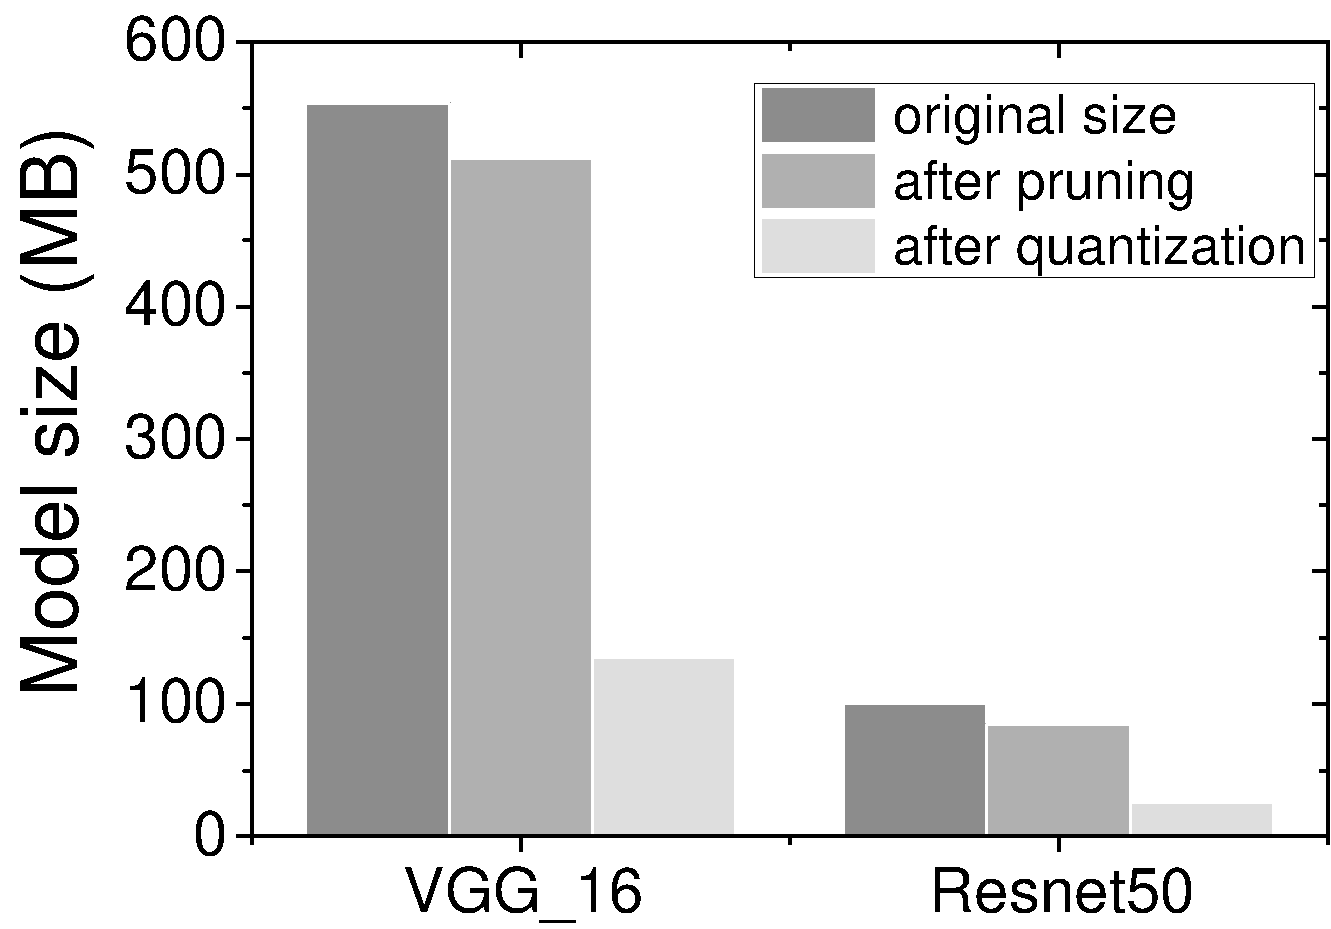
\includegraphics[width=0.3\textwidth]{figure/motivation_size.pdf}}
\hfill
\subfloat[][Inference time]{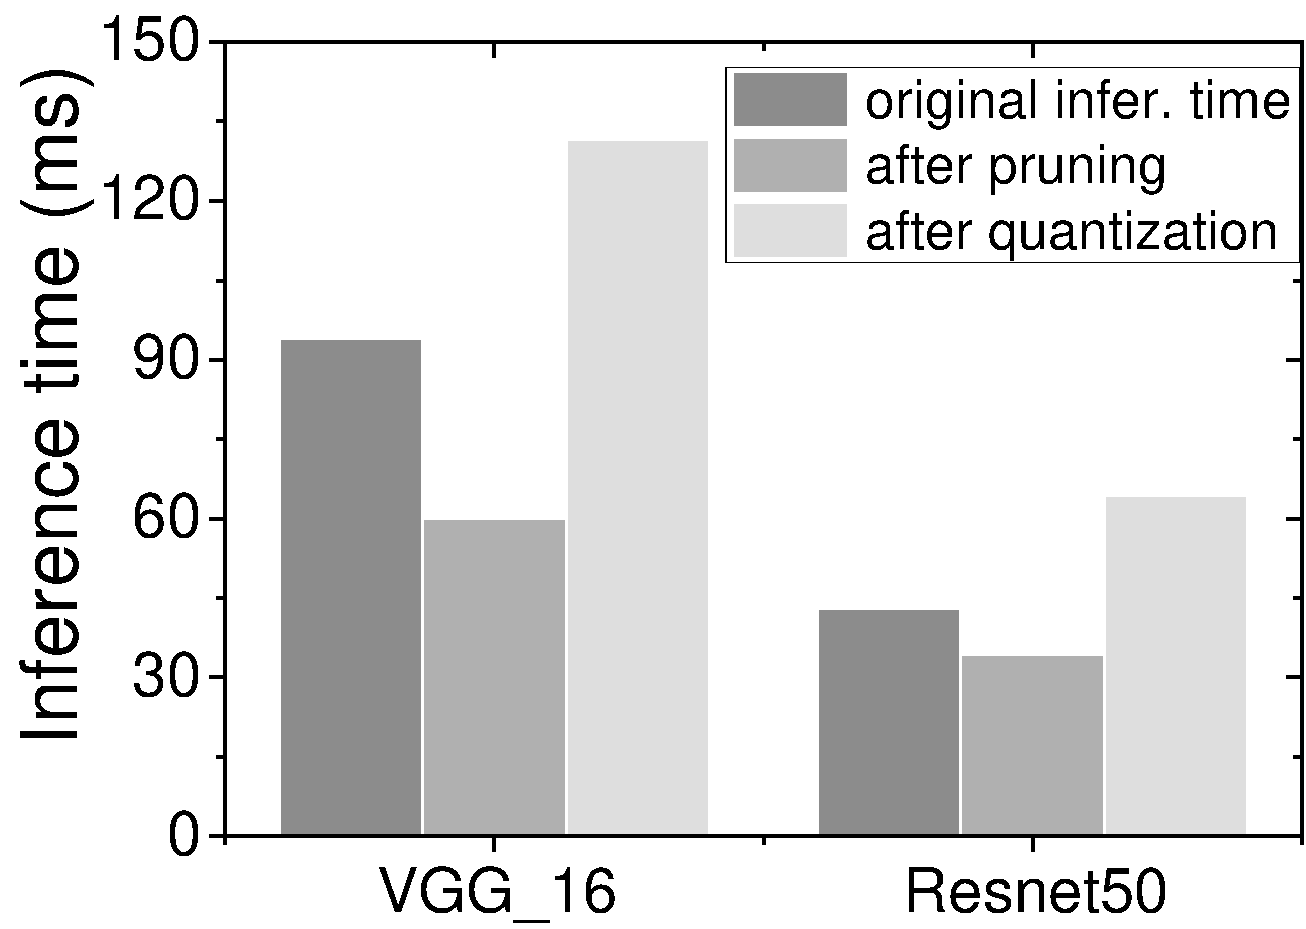
\includegraphics[width=0.3\textwidth]{figure/motivation_time.pdf}}
\hfill
\subfloat[][Accuracy]{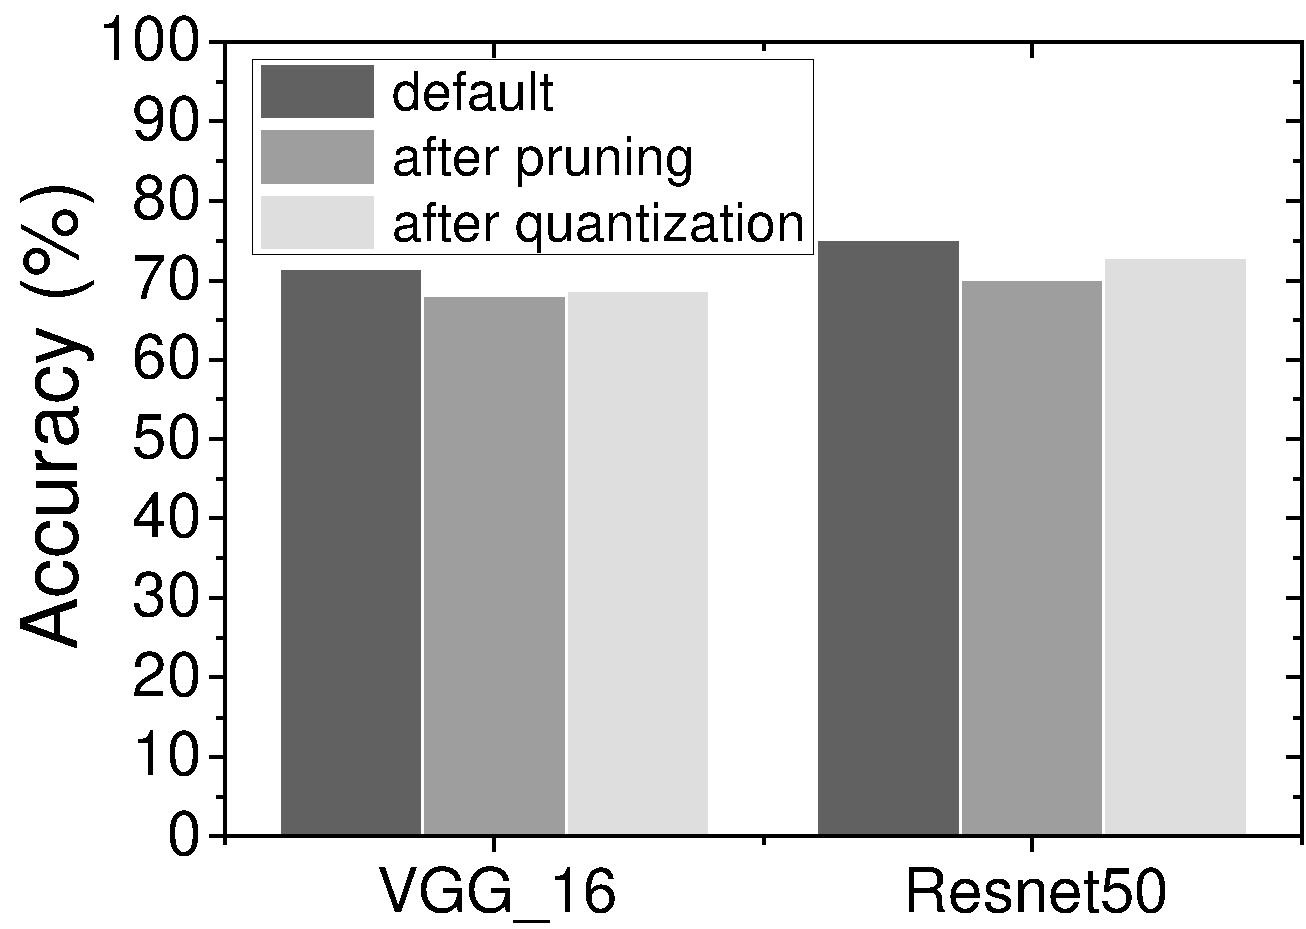
\includegraphics[width=0.3\textwidth]{figure/motivation_accuracy.pdf}}
\caption{The achieved model size (a) inference time (b) and accuracy (c) before and after the compression by quantization and pruning.
There is significant room for improvement.}
\label{fig:motivation}
\end{figure}